\section{Resultados}

Este tópico é dedicado a apresentar os resultados, adversidades e contribuições 
alcançadas durante o desenvolvimento do estudo referente ao problema proposto. 
Por fim, são apresentadas considerações sobre as limitações ocorridas no 
desenvolvimento deste trabalho. Nos resultados do problema proposto, este 
estudo utilizou as principais métricas da literatura para análise de desempenho 
dos classificadores.

\subsection{Disposição das classes nos \textit{datasets} \textbf{A} e \textbf{B}}

No caso dos \textit{datasets}, ambos dispõem de 250 redações cada, com temas 
diversificados que passaram por um processo de avaliação manual com diferentes 
avaliadores. O Gráfico \ref{graphic:class_dataset_balanced} demonstra a 
disposição das classes distintas (0.00, 0.50, 1.00, 1.50, 2.00) sobre a 
competência II, respectivamente de (\textbf{A}, \textbf{B}).

\begin{figure}[H]
    \begin{center}
    \begin{tikzpicture}
        \begin{axis}[
                ybar,
                width=15cm,
                height=10cm,
                symbolic x coords={0.00,0.50,1.00,1.50,2.00},
                legend style={at={(0.7,0.9)},anchor=north west},
                bar width=8pt,
                ylabel=Quantidade,
                xlabel=Classes,
                xtick=data,
                axis lines*=left,
            ]
            \addlegendentry{Dataset A}
            \addplot[draw=blue] coordinates{
                (0.00,50)
                (0.50,50)
                (1.00,50)
                (1.50,50)
                (2.00,50)
            };
            \addlegendentry{Dataset B}
            \addplot[draw=red] coordinates{
                (0.00,50)
                (0.50,50)
                (1.00,50)
                (1.50,50)
                (2.00,50)
            };
            \node [above] at (axis cs:  0.00,50) {50};
            \node [above] at (axis cs:  0.50,50) {50};
            \node [above] at (axis cs:  1.00,50) {50};
            \node [above] at (axis cs:  1.50,50) {50};
            \node [above] at (axis cs:  2.00,50) {50};
        \end{axis}
    \end{tikzpicture}
    \caption{Distribuição das classes sobre a competência II de 250 redações dos 
    \textit{datasets} \textbf{A} e \textbf{B}}
    \label{graphic:class_dataset_balanced}
    \end{center}
\end{figure}

Ambos os \textit{datasets} possuem uma amostragem reduzida devido a aplicação da 
técnica de subamostragem \textit{undersampling}, que remove os elementos da 
classe majoritária de forma aleatória, a fim de promover o balanceamento. 
Além disso, \citeauthoronline{machado2009estudo} (\citeyear{machado2009estudo}) 
em seu estudo indica o uso das técnicas de limpeza de dados a fim de eliminar 
os exemplos ruidosos e \textit{limítrofes}, respectivamente 
(\textit{class-label noise}, \textit{borderlines}). A quantidade de exemplos 
pode apresentar-se de uma certa forma modesta, porém normalmente ela é 
suficientemente para a inferência indutiva.

\subsection{Resultado da inferência indutiva do dataset A}
% É apresentado os resultados 
% da inferência indutiva dos classificadores sobre cada \textit{dataset} a fim de
% validar a hipótese de recuperação de padrões na valoração textual.

% Nos resultados do problema proposto, este estudo utilizou as principais métricas 
% da literatura para análise de desempenho dos classificadores, tendo como foco 
% as métricas: \textit{Acurácia} Curva ROC, e Matriz de Confusão.

A inferência indutiva dos classificadores \textit{Adabost} e 
\textit{Naive Bayes}, utilizando o \textit{dataset} \textbf{A} originou o 
Gráfico \ref{graphic:dataset_a_acuracia}, onde está delineado os resultados da 
\textit{acurácia} de cada classe distinta sobre domínio do problema. Com isso, 
nota-se que em relação ao algoritmo \textit{Adaboost}, a indução do 
\textit{Naive Bayes} proveu uma melhor acurácia na maior parte das classes.

% Acurácia dataset A
\begin{figure}[H]
    \begin{center}
        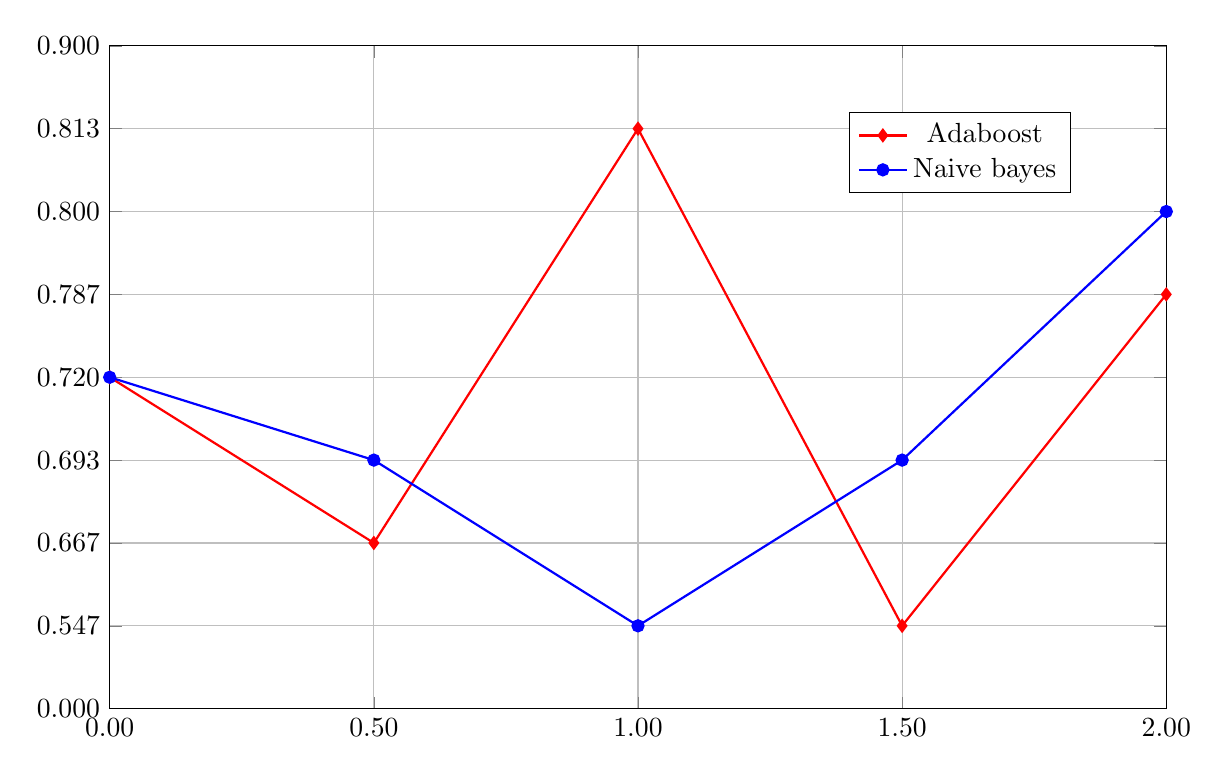
\begin{tikzpicture}
        \begin{axis}[width=15cm, 
            height=10cm, 
            grid=both, 
            ymin=0.000,
            ymax=0.900,
            xmax=2.00,
            xmin=0.00, 
            legend style={at={(0.7,0.9)},anchor=north west},
            symbolic x coords={0.00, 0.50, 1.00, 1.50, 2.00}, 
            symbolic y coords={0.000, 0.547,0.667,0.693,0.720,0.787,0.800,0.813, 0.900},
            xtick=data]

        \addlegendentry{Adaboost}
        \addplot[mark=diamond*,thick,red] coordinates {
        (0.00,0.720) 
        (0.50,0.667) 
        (1.00,0.813) 
        (1.50,0.547) 
        (2.00,0.787) 
        };

        \addlegendentry{Naive bayes}
        \addplot[mark=*,thick,blue] coordinates {
        (0.00,0.720) 
        (0.50,0.693) 
        (1.00,0.547) 
        (1.50,0.693) 
        (2.00,0.800) 
        };
        \end{axis}
        \end{tikzpicture}
    \end{center}
    \caption{Sobreposição dos resultados de \textit{acurácia} da inferência  
    indutiva dos algoritmos \textit{Adaboost} e \textit{Naive Bayes} sobre 
    o \textit{dataset} A}
    \label{graphic:dataset_a_acuracia}
\end{figure}

No Gráfico \ref{graphic:dataset_a_roc} é apresentado os resultados referentes 
ao ponto de corte da curva ROC correspondente a cada classe distinta. Através 
deste ponto avalia-se o poder de discriminação das classes. 

% Curva ROC dataset A
\begin{figure}[H]
    \begin{center}
        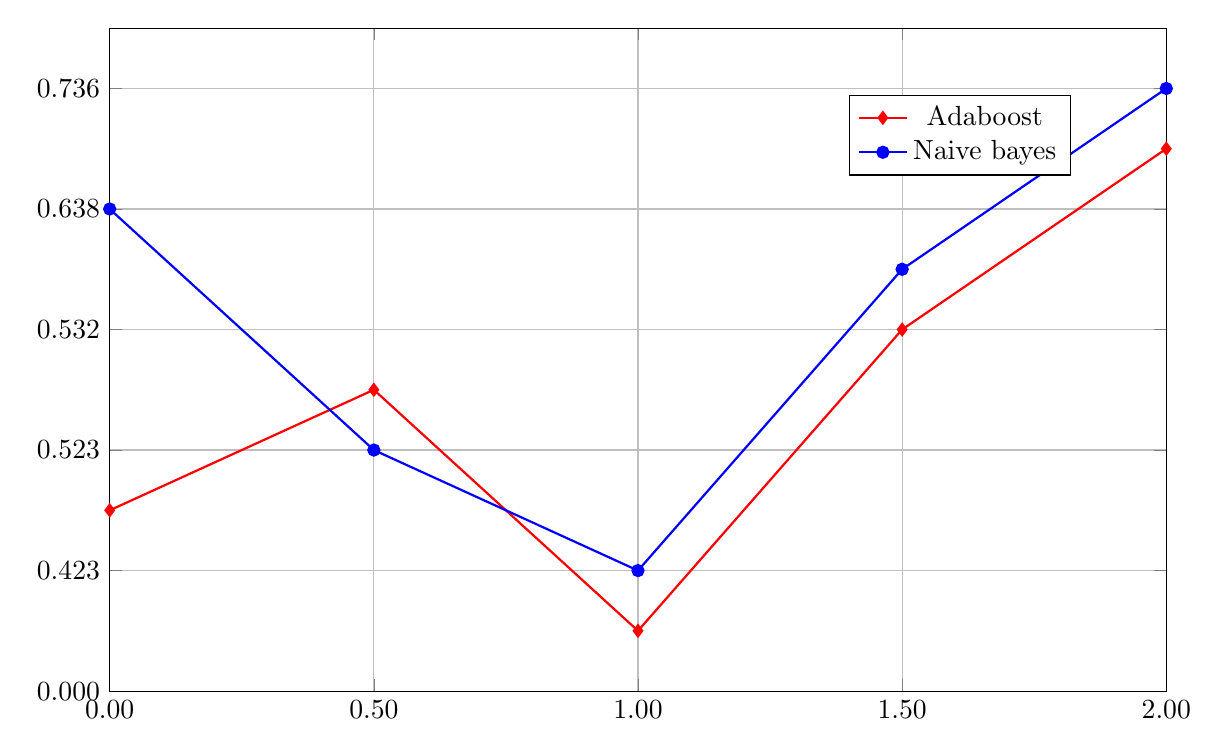
\begin{tikzpicture}
        \begin{axis}[width=15cm, 
            height=10cm, 
            grid=both, 
            ymin=0.000,
            ymax=0.900,
            xmax=2.00,
            xmin=0.00, 
            legend style={at={(0.7,0.9)},anchor=north west},
            symbolic x coords={0.00, 0.50, 1.00, 1.50, 2.00}, 
            symbolic y coords={0.000, 0.419,0.423,0.475,0.523,0.531,0.532,0.577,0.638,0.657,0.736, 0.900},
            xtick=data]

        \addlegendentry{Adaboost}
        \addplot[mark=diamond*,thick,red] coordinates {
        (0.00,0.475) 
        (0.50,0.531) 
        (1.00,0.419) 
        (1.50,0.532) 
        (2.00,0.657) 
        };

        \addlegendentry{Naive bayes}
        \addplot[mark=*,thick,blue] coordinates {
        (0.00,0.638) 
        (0.50,0.523) 
        (1.00,0.423) 
        (1.50,0.577) 
        (2.00,0.736) 
        };
        \end{axis}
        \end{tikzpicture}
    \end{center}
    \caption{Rurva roc}
    \label{graphic:dataset_a_roc}
\end{figure}

% Matriz de confusão Adaboost dataset A
\begin{table}[H]
    \centering
    \begin{tabular}{cc|c|c|c|c|c|c|}
    \cline{3-8}
     &  & \multicolumn{6}{c|}{\textbf{Adaboost}} \\ \cline{3-8} 
     &  & \textbf{0.00} & \textbf{0.50} & \textbf{1.00} & \textbf{1.50} & \textbf{2.00} & $\sum_{}$  \\ \hline
    \multicolumn{1}{|c|}{} & \textbf{0.00} & \textbf{3} & 1 & 4 & 2 & 0 & \textit{10} \\ \cline{2-8} 
    \multicolumn{1}{|c|}{} & \textbf{0.50} & 2 & \textbf{8} & 5 & 1 & 4 & \textit{20} \\ \cline{2-8} 
    \multicolumn{1}{|c|}{} & \textbf{1.00} & 3 & 6 & \textbf{2} & 5 & 3 & \textit{19} \\ \cline{2-8} 
    \multicolumn{1}{|c|}{} & \textbf{1.50} & 4 & 4 & 3 & \textbf{0} & 2 & \textit{13} \\ \cline{2-8} 
    \multicolumn{1}{|c|}{} & \textbf{2.00} & 5 & 2 & 0 & 2 & \textbf{4} & \textit{13} \\ \cline{2-8} 
    \multicolumn{1}{|c|}{\multirow{-6}{*}{\rot{Atual}}} & $\sum_{}$ & \textit{17} & \textit{21} & \textit{14} & \textit{10} & \textit{13} & \textit{75} \\ \hline
    \end{tabular}
    \caption{Tabela de contingência ou Matriz de confusão resultante da indução do classificador AdaBoost.}
    \label{tab:matrix_adaboost_a}
\end{table}

% Matriz de confusão Naive Bayes dataset A
\begin{table}[H]
    \centering
    \begin{tabular}{cc|c|c|c|c|c|c|}
    \cline{3-8}
     &  & \multicolumn{6}{c|}{\textbf{Naive Bayes}} \\ \cline{3-8} 
     &  & \textbf{0.00} & \textbf{0.50} & \textbf{1.00} & \textbf{1.50} & \textbf{2.00} & $\sum_{}$  \\ \hline
    \multicolumn{1}{|c|}{} & \textbf{0.00} & \textbf{1} & 5 & 3 & 0 & 1 & \textit{10} \\ \cline{2-8} 
    \multicolumn{1}{|c|}{} & \textbf{0.50} & 0 & \textbf{9} & 8 & 1 & 2 & \textit{20} \\ \cline{2-8} 
    \multicolumn{1}{|c|}{} & \textbf{1.00} & 0 & 10 & \textbf{6} & 2 & 1 & \textit{19} \\ \cline{2-8} 
    \multicolumn{1}{|c|}{} & \textbf{1.50} & 1 & 2 & 2 & \textbf{3} & 5 & \textit{13} \\ \cline{2-8} 
    \multicolumn{1}{|c|}{} & \textbf{2.00} & 0 & 4 & 4 & 4 & \textbf{1} & \textit{13} \\ \cline{2-8} 
    \multicolumn{1}{|c|}{\multirow{-6}{*}{\rot{Atual}}} & $\sum_{}$ & \textit{2} & \textit{30} & \textit{23} & \textit{10} & \textit{10} & \textit{75} \\ \hline
    \end{tabular}
    \caption{Tabela de contingência ou Matriz de confusão resultante da indução do classificador AdaBoost.}
    \label{tab:matrix_naive_a}
\end{table}

\subsection{Resultado da inferência indutiva do dataset B}

% Acurácia dataset B
\begin{figure}[H]
    \begin{center}
        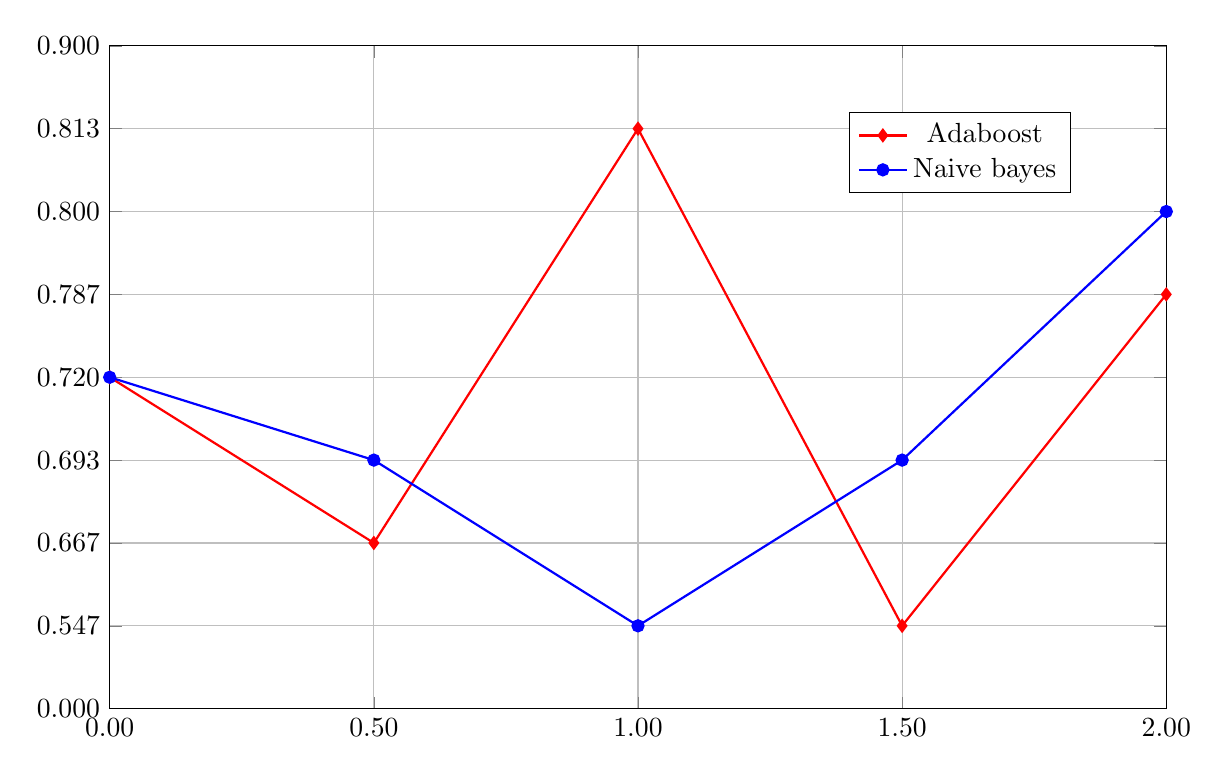
\begin{tikzpicture}
        \begin{axis}[width=15cm, 
            height=10cm, 
            grid=both, 
            ymin=0.000,
            ymax=0.900,
            xmax=2.00,
            xmin=0.00, 
            legend style={at={(0.7,0.9)},anchor=north west},
            symbolic x coords={0.00, 0.50, 1.00, 1.50, 2.00}, 
            symbolic y coords={0.000, 0.547,0.667,0.693,0.720,0.787,0.800,0.813, 0.900},
            xtick=data]

        \addlegendentry{Adaboost}
        \addplot[mark=diamond*,thick,red] coordinates {
        (0.00,0.720) 
        (0.50,0.667) 
        (1.00,0.813) 
        (1.50,0.547) 
        (2.00,0.787) 
        };

        \addlegendentry{Naive bayes}
        \addplot[mark=*,thick,blue] coordinates {
        (0.00,0.720) 
        (0.50,0.693) 
        (1.00,0.547) 
        (1.50,0.693) 
        (2.00,0.800) 
        };
        \end{axis}
        \end{tikzpicture}
    \end{center}
    \caption{Acurácia}
    \label{graphic:dataset_a_acuracia}
\end{figure}

% Curva ROC dataset B
\begin{figure}[H]
    \begin{center}
        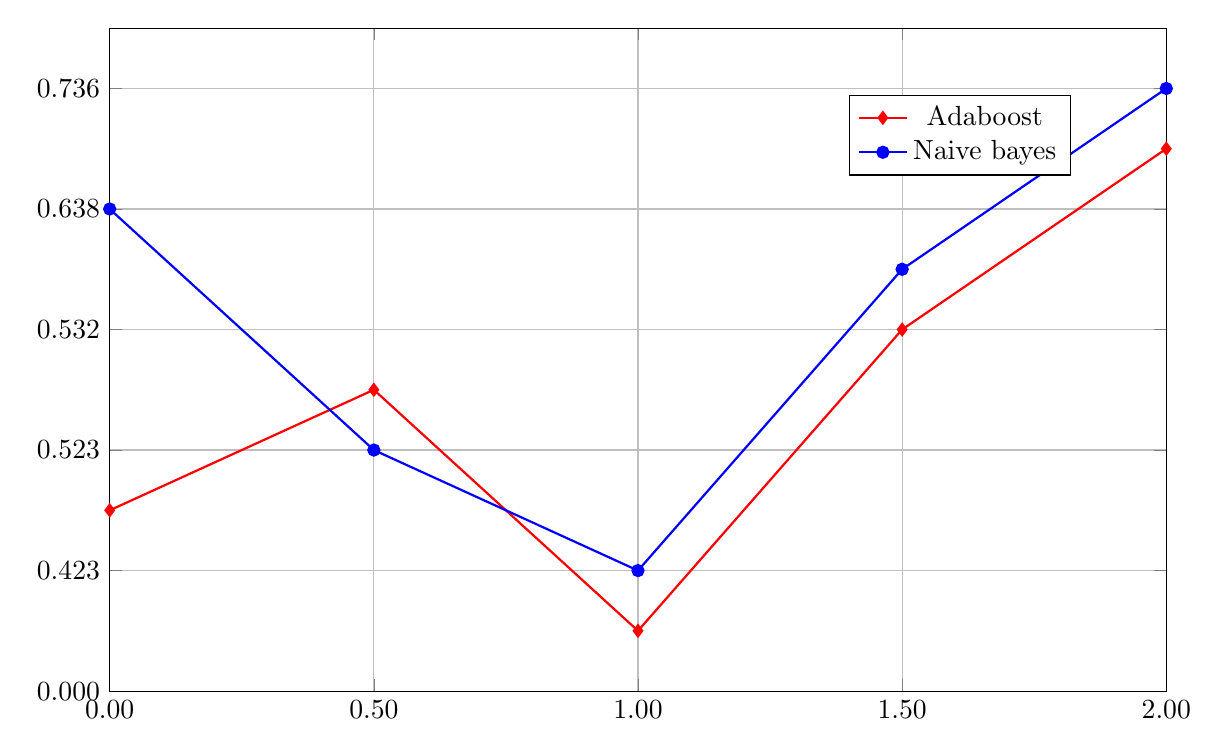
\begin{tikzpicture}
        \begin{axis}[width=15cm, 
            height=10cm, 
            grid=both, 
            ymin=0.000,
            ymax=0.900,
            xmax=2.00,
            xmin=0.00, 
            legend style={at={(0.7,0.9)},anchor=north west},
            symbolic x coords={0.00, 0.50, 1.00, 1.50, 2.00}, 
            symbolic y coords={0.000, 0.419,0.423,0.475,0.523,0.531,0.532,0.577,0.638,0.657,0.736, 0.900},
            xtick=data]

        \addlegendentry{Adaboost}
        \addplot[mark=diamond*,thick,red] coordinates {
        (0.00,0.475) 
        (0.50,0.531) 
        (1.00,0.419) 
        (1.50,0.532) 
        (2.00,0.657) 
        };

        \addlegendentry{Naive bayes}
        \addplot[mark=*,thick,blue] coordinates {
        (0.00,0.638) 
        (0.50,0.523) 
        (1.00,0.423) 
        (1.50,0.577) 
        (2.00,0.736) 
        };
        \end{axis}
        \end{tikzpicture}
    \end{center}
    \caption{Rurva roc}
    \label{graphic:dataset_a_roc}
\end{figure}

% Matriz de confusão Adaboost dataset B
\begin{table}[H]
    \centering
    \begin{tabular}{cc|c|c|c|c|c|c|}
    \cline{3-8}
     &  & \multicolumn{6}{c|}{\textbf{Predição}} \\ \cline{3-8} 
     &  & \textbf{0.00} & \textbf{0.50} & \textbf{1.00} & \textbf{1.50} & \textbf{2.00} & $\sum_{}$  \\ \hline
    \multicolumn{1}{|c|}{} & \textbf{0.00} & 4 & 18 & 13 & 2 & 0 & \textbf{37} \\ \cline{2-8} 
    \multicolumn{1}{|c|}{} & \textbf{0.50} & 13 & 42 & 44 & 14 & 1 & \textbf{114} \\ \cline{2-8} 
    \multicolumn{1}{|c|}{} & \textbf{1.00} & 18 & 51 & 78 & 32 & 11 & \textbf{190} \\ \cline{2-8} 
    \multicolumn{1}{|c|}{} & \textbf{1.50} & 7 & 14 & 31 & 15 & 2 & \textbf{69} \\ \cline{2-8} 
    \multicolumn{1}{|c|}{} & \textbf{2.00} & 4 & 2 & 14 & 3 & 3 & \textbf{26} \\ \cline{2-8} 
    \multicolumn{1}{|c|}{\multirow{-6}{*}{\rot{Atual}}} & $\sum_{}$ & \textbf{46} & \textbf{127} & \textbf{180} & \textbf{66} & \textbf{17} & \textbf{436} \\ \hline
    \end{tabular}
    \caption{Tabela de contingência ou Matriz de confusão resultante da indução do classificador AdaBoost.}
    \label{tab:matrix_adaboost_b}
\end{table}

% Matriz de confusão Naive Bayes dataset B
\begin{table}[H]
    \centering
    \begin{tabular}{cc|c|c|c|c|c|c|}
    \cline{3-8}
     &  & \multicolumn{6}{c|}{\textbf{Predição}} \\ \cline{3-8} 
     &  & \textbf{0.00} & \textbf{0.50} & \textbf{1.00} & \textbf{1.50} & \textbf{2.00} & $\sum_{}$  \\ \hline
    \multicolumn{1}{|c|}{} & \textbf{0.00} & 4 & 18 & 13 & 2 & 0 & \textbf{37} \\ \cline{2-8} 
    \multicolumn{1}{|c|}{} & \textbf{0.50} & 13 & 42 & 44 & 14 & 1 & \textbf{114} \\ \cline{2-8} 
    \multicolumn{1}{|c|}{} & \textbf{1.00} & 18 & 51 & 78 & 32 & 11 & \textbf{190} \\ \cline{2-8} 
    \multicolumn{1}{|c|}{} & \textbf{1.50} & 7 & 14 & 31 & 15 & 2 & \textbf{69} \\ \cline{2-8} 
    \multicolumn{1}{|c|}{} & \textbf{2.00} & 4 & 2 & 14 & 3 & 3 & \textbf{26} \\ \cline{2-8} 
    \multicolumn{1}{|c|}{\multirow{-6}{*}{\rot{Atual}}} & $\sum_{}$ & \textbf{46} & \textbf{127} & \textbf{180} & \textbf{66} & \textbf{17} & \textbf{436} \\ \hline
    \end{tabular}
    \caption{Tabela de contingência ou Matriz de confusão resultante da indução do classificador AdaBoost.}
    \label{tab:matrix_naive_b}
\end{table}





% \begin{figure}[H]
%     \begin{center}
%         \begin{tikzpicture}
%         \begin{axis}[width=15cm, 
%             height=10cm, 
%             grid=both, 
%             ymin=0.000,
%             ymax=0.900,
%             xmax=2.00,
%             xmin=0.00, 
%             legend style={at={(0.7,0.9)},anchor=north west},
%             symbolic x coords={0.00, 0.50, 1.00, 1.50, 2.00}, 
%             symbolic y coords={0.000, 0.419,0.423,0.475,0.523,0.531,0.532,0.547,0.577,0.638,0.657,0.667,0.693,0.720,0.736,0.787,0.800,0.813, 0.900},
%             xtick=data]

%         \addlegendentry{Acurácia Adaboost}
%         \addplot[mark=triangle*,thick,blue] coordinates {
%         (0.00,0.720) 
%         (0.50,0.693) 
%         (1.00,0.547) 
%         (1.50,0.693) 
%         (2.00,0.800) 
%         };

%         \addlegendentry{Acurácia Naive Bayes}
%         \addplot[mark=diamond*,thick,blue] coordinates {
%         (0.00,0.720) 
%         (0.50,0.667) 
%         (1.00,0.813) 
%         (1.50,0.547) 
%         (2.00,0.787) 
%         };
        
%         \addlegendentry{Curva ROC Adaboost}
%         \addplot[mark=diamond*,thick,red] coordinates {
%         (0.00,0.475) 
%         (0.50,0.531) 
%         (1.00,0.419) 
%         (1.50,0.532) 
%         (2.00,0.657) 
%         };

%         \addlegendentry{Curva ROC Naive bayes}
%         \addplot[mark=*,thick,red] coordinates {
%         (0.00,0.638) 
%         (0.50,0.523) 
%         (1.00,0.423) 
%         (1.50,0.577) 
%         (2.00,0.736) 
%         };

%         \end{axis}
%         \end{tikzpicture}
%     \end{center}
%     \caption{Rurva roc}
%     \label{graphic:dataset_a_roc_teste}
% \end{figure}







